%% Copyright 2019 Bernd Haberstumpf
%% License: CC BY-NC
% !TeX spellcheck = de_DE
\newsection{Regelsystem}

Die Rollenspielregeln sind auf den narrativen Charakter des Plots ausgelegt. Es handelt sich um ein W6 W"urfelsystem bei dem vier W"urfel pro Spieler bzw.~den Spielleiter ausreichen. W"urfel legen dabei nicht die Eigenschaften einen Charakter im Detail fest oder beschreiben das Ergebnis einer Aktion, sondern spei\3en lediglich einen Zufallsfaktor in das Ergebnis ein. Das Ergebnis einer Aktion oder auch eines Ereignisses legt der Spielleiter unter Ber"ucksichtigung der Handlungen und des W"urfelergebnisses selbst fest. Das Regelsystem ist angelehnt an den Konzepten des Rollenspiels "`Blades in the Dark"'.


\newsection{W"urfelw"urfe}

Der Erfolg von Aktionen wird wie Beschrieben durch W"urfel beeinflusst werden. Das W"urfelergebins beschreibt wie erfolgreich eine Aktion gewesen ist. W"urfelw"urfe werden mit einem bis drei W6 W"urfeln ausgetragen. Das h"ochste W"urfelergebnis z"ahlt.

Es wird unterschieden zwischen \emph{Alltagswurf}, \emph{Einfacher Wurf}, \emph{Risikowurf} und \emph{Vergleichender Wurf}.

\subsection{Alltagswurf}
Ein Alltagswurf kann bei einer allt"aglichen Situation zum Einsatz kommen wie z.B. im ComNetz suchen. Bei einem Alltagswurf werden drei W"urfelerebnisse unterschieden:

\begin{diceroles}
    \sdice{1} & Die Aktion ist fehlgeschlagen und hat negative Auswirkungen auf den Ausf"uhrenden. \\
    \rdice{2}{5} & Die Aktion hatte Erfolg. \\
    \sdice{6} & Die Aktion hat einen herausragendes Erfolg. \\
\end{diceroles}

\begin{ruleexample}
    Rondra ist auf der Suche nach Informationen in einer einschl"agigen Disko. Sie begiebt sich auf die Tanzfl"ache. Der Spielleiter entscheidet sich f"ur einen W"urfelwurf. Rondra w"urfelt:

    \begin{diceroles}
        \sdice{1} & Rondra rempelt mehrere Discobesucher an und ger"at damit ins Visier der Security. \\
        \rdice{2}{5} & Rondra tanzt ungezwungen und kann dabei andere Discobesucher ansprechen. \\
        \sdice{6} & Rondra legt eine beeindruckende Performance aufs Parkett und erregt das Interesse des Barmanns Bruno 
            der ihr nur allzu gerne Antworten auf ihre Fragen gibt. \\
    \end{diceroles}
\end{ruleexample}

\subsection{Einfacher Wurf}
Ein einfacher Wurf beeinflusst das Ergebnis einer nicht allt"aglichen Herausforderung. Folgende W"urfelergebnisse werden unterschieden:

\begin{diceroles}
    \sdice{1} &  Die Aktion ist schwerwiegend fehlgeschlagen und hat negative Auswirkungen auf den der die Aktion ausf"uhren wollte.\\
    \rdice{2}{3} & Die Aktion hatte keinen Erfolg. \\
    \rdice{4}{5} & Die Aktion hatte einen Teilerfolg. \\
    \sdice{6} & Die Aktion hatte vollen Erfolg.\\
\end{diceroles}

\begin{ruleexample}
    Hektor ist auf der Suche nach Informationen im Raumhafen von Valhalla. Er wird von dem Agenten Johnson beschattet. Der Spielleiter l"asst den Spieler w"urfeln. Wird er den Agenten als solchen erkennen?

    \begin{diceroles}
        \sdice{1} & Der Agent rempelt Hektor unerkannt an und heftet ihm eine Nanowanze an den Overall.\\
        \rdice{2}{3} & Hektor bemerkt nichts.\\
        \rdice{5}{6} & Hektor bemerkt, dass er verfolgt wird verliert den Agenten zun"achst wieder aus den Augen.\\
        \sdice{6} & Hektor hat den Agenten entdeckt ohne das dieser seine Entdeckung bemerkt hat.\\
    \end{diceroles}
\end{ruleexample}

\subsection{Risikowurf}
Ein Risikowurf ist ein W"urfelwurf bei dem der W"urfelnde geringen Chancen auf Erfolg hat. Folgende W"urfelergebnisse kommen in Betracht:

\begin{diceroles}
    \sdice{1} & Die Aktion ist schwerwiegend fehlgeschlagen und hat negative Auswirkungen auf den der die Aktion ausf"uhren wollte.\\
    \rdice{2}{5} & Die Aktion hatte keinen Erfolg.\\
    \sdice{6} & Die Aktion hat einen Teilerfolg erzielt.\\
    \tdice{6}{6} & Die Aktion hat einen vollen Erfolg.\\
\end{diceroles}

\begin{ruleexample}
    In einem Raumgefecht erleidet Hektors Shuttle einen Schaden an der Man"ovriereinheit und taumelt durchs All. Haktor beschie\3t den Schaden an der Bordwand zu reparieren und verl"asst im Raumanzug das innere des Schiffs. Der Spielleiter l"asst w"urfeln:
    
    \begin{diceroles}
        \sdice{1} & Hektors Magnetstiefel verlieren die Haftung auf der Bordwand und Hektor schl"agt mit dem Kopf auf. Nun h"angt er  
            bewusstlos am Rettungsseil. Hoffentlich ist noch eine zweite Person an Bord, die ihn retten kann. \\
        \rdice{2}{5} & Hektor kann den Schaden nicht beheben.\\
        \sdice{6} & Hektor schafft es einen Teil der Steuereinheit notd"urftig zu reparieren. Hoffentlich reicht es das Schiff aus 
            der Schu\3linie zu bringen.\\
        \tdice{6}{6} & Hektor kann die Steuereinheit wieder vollst"andig in Betrieb nehmen.\\
    \end{diceroles}
\end{ruleexample}

\subsection{Vergleichender Wurf}
Bei einem vergleichenden Wurf kann das Ergebnis des ersten Wurfs durch einen Gegenwurf negativ beeinflusst werden. Ein vergleichender Wurf ist z.B. ein Angriff und eine Verteidigung. Der Angriffserfolg kann durch den verteidigenden Wurf abgeschw"acht werden. Erfolge eines verteidigenden Wurfs haben folgenden Einflu\3:

\begin{center}\begin{tabular}{m{1.2cm} m{1.2cm} m{11cm}}
    \textbf{Anriff} & \textbf{Vert.} & \textbf{Auswirkung} \\\hline
    Voll & Voll & Teilerfolg \\
    Voll & Teil & Minderung schwerer Folgen \\
    Teil & Voll & kein Erfolg \\
    Teil & Teil & Minderung Teilerfolg \\
\end{tabular}\end{center}

\begin{ruleexample}
    Hektor hat den Agenten Johnson potentiell im Raumhafen entdeckt. Johnson ist sich der Gefahr bewusst und will sich der Entdeckung entziehen. Der Spielleiter entscheidet sich f"ur einen vergleichenden Wurf.

    \begin{center}\begin{tabular}{m{1.2cm} m{1.2cm} m{11cm}}
        \textbf{Anriff} & \textbf{Vert.} & \textbf{Auswirkung} \\\hline
        Voll & Voll & Hektor bemerkt, dass er verfolgt verliert den Agenten aber wieder unerkannt aus den Augen.  \\
        Voll & Teil & Hektor hat den Agenten entdeckt, der Agent bemerkt, dass er aufgeflogen ist.\\
        Teil & Voll & Hektor bemerkt nichts. \\
        Teil & Teil & Hektor hat das Gef"uhl das er verfolgt wird. \\
    \end{tabular}\end{center}
\end{ruleexample}

\newsection{Der Charakter}

Die F"ahigkeiten und Eigenschaften eines Charakter sind neben den menschlichen Grundf"ahigkeiten durch seinen Hintergrund und spezielle St"arken und Schw"achen bestimmt. 

\begin{description}
    \item[Grundf"ahigkeiten] sind F"ahigkeiten die jeder Humanoiden mehr oder weniger beherrscht. Alles wof"ur keine spezielle Ausbildung,  
        kein spezielles ethnischer oder kulturelles Hintergrundwissen und keine speziellen K"orpereigenschaften ben"otigt werden f"allt in diese Kategorie. Jeder der es bis ins All geschafft hat kann Lesen schreiben und rechnen. Auch kann jeder eine entsicherte Feuerwaffen abfeuern. Auch k"onnen sich alle Bewohner der au\3erterrestrischen Kolonien miteinander irgendwie unterhalten. Gesprochen wird ein Kauderwelsch aus Englisch mit starken Einfl"ussen von Russisch, Chinesisch und Spanisch. Ausfl"uge mit einem Raumanzug ins All sind hingegen nicht selbstverst"andlich.  Aktionen in einer Grundf"ahigkeit werden mit \textbf{1W6} gew"urfelt. 
    \item[Hintergr"unde] beginnen mit einer Kulturkreis entsprechender Muttersprache fortgef"uhrt durch Schulbildung und Profession mit 
        entsprechendem Wissen und entsprechenden F"ahigkeiten wie auch Kontakten. Der Hintergrund erweitert Grundf"ahigkeiten Charakter individuell. Hintergr"unde werden ebenfalls mit \textbf{1W6} gew"urfelt. Was die Hintergr"unde eines Charakters umfassen kann Szenen individuell durch den Spielleiter passend zum Spielverlauf bestimmt werden. Wenn der Spieler "uberzeugend darlegen. Kann der Spieler aufgrund seines Hintergrunds glaubhaft darlegen, dass er eine F"ahigkeit beherrscht kann er diese anwenden.
    \item[St"arken] beschreiben in was ein Charakter besonders gut kann. St"arken erlauben mit zus"atzlich W"urfeln zu w"urfeln. 
    \item[Talente \& Schw"achen] Talente sind besondere Talente wie eine fotograpisches Ged"achtnis. Schw"achen k"onnen k"orperliche  
        Gebrechen, Phobien, Unbeherrschtheit eine Sucht aber auch eine rachs"uchtige Exfreundin sein. Sie k"onnen durch den Spielleiter oder auch den Spieler eingesetzt werden um dem Charakter mehr pers"onliche Tiefe zu geben.
\end{description}        

\newsection{Die Helden}

Eine Rollenspielkampagne entspricht einer Actionserie bei der die Spieler die Rollen der Helden "ubernehmen. Als Held treten die Charaktere aus der Masse der Normalsterblichen heraus. Helden k"onnen ausweglosen Situationen meistern, denn sie haben Gl"uck, mehr Gl"uck als normale Personen. Im Regelwerk wird das Gl"uck durch \emph{Schicksalspunkte} repr"asentiert die w"ahrend des Spiels ausgegeben werden k"onnen. Schicksalspunkte werden nach jeder Szene wieder auff"ullen. Das Ausgeben eines Schicksalspunktes erlaubt es dem Spieler einen oder mehrere \textbf{W"urfel noch einmal zu w"urfeln} oder alternativ \textbf{einen W"urfel mehr} zu w"urfeln. Ein W"urfelwurf darf dabei allerdings maximal mit drei W"urfeln, bei Anwendung von Waffen oder R"ustungen mit view W"urfeln ausgef"uhrt werden.

Die Helden sind im Normalfall auch keine ungebildeten Tagel"ohner. Sie besitzen eine gute Ausbildung, Kontakte und Resourcen. K"orpermodifikationen wie ein Commandchip d"urfen vorausgesetzt werden. Helden sind zumindest rudiment"are mit dem Umgang eines Raumanzugs vertraut.

Helden sind z"ah. Wie in einem Roman stehen Helden in jeder neuen Szene auf der Matte um die n"achste Herausforderung zu meistern. Die Szenen in einer Geschichte sind meist so gestaltet, dass dazwischen Zeit vergeht und die Charaktere sich in einer sicheren Umgebung aufhalten k"onnen. So k"onnen sie sich erholen. St"arkere Verletzungen die ein weiterspielen behindern oder unglaubw"urdig machen k"onnen in einer sicheren Umgebung geheilt werden. Die Medizin hat sich in den zuk"unftigen 200 Jahren stark weiterentwickelt. KI getst"utze Autobots assistieren bei medizinischen Eingriffen oder f"uhren Operationen durch. Innere Organe lassen sich durch k"unstliche Organe ersetzen. Gez"uchtete und k"unstliche Gliedma\3en lassen nat"urliche Gliedma\3en voll funktionsf"ahig ersetzen. Mikrobenkulturen erlauben verletzte zu stabilisieren.

\newsection{Charakter Erschaffung}

Die F"ahigkeiten und Eigenschaften eines Charakters werden bei der Erstellung des Charakters festgelegt und auf seinem Charakter Datenblatt festgehalten. Das Charakter Datenblatt ist am Ende dieses Kapitel angeh"angt und kann separat im Internet herunter geladen werden. Ein entsprechender Link findet sich unter Quallenangaben am Ende des Buchs. Charakter Datenbl"atter sind "ublicherweise in englischer Sprache. Das bei diesem Regelsytem ebenfalls der Fall.

\begin{column}[l]{0.52}
    Das Charakter Datenblatt beginnt mit allgemeinen Informationen wie Name, Geschlecht (\emph{GENDER}), Rasse (\emph{RACE}), Alter (\emph{AGE}), Talente und Schw"achen (\emph{MERITS \& FLAWS}). Die ver"ugbaren Rassen sind im n"achsten Kapitel beschrieben.
\end{column}
\begin{column}[r]{0.48}
    \centering
    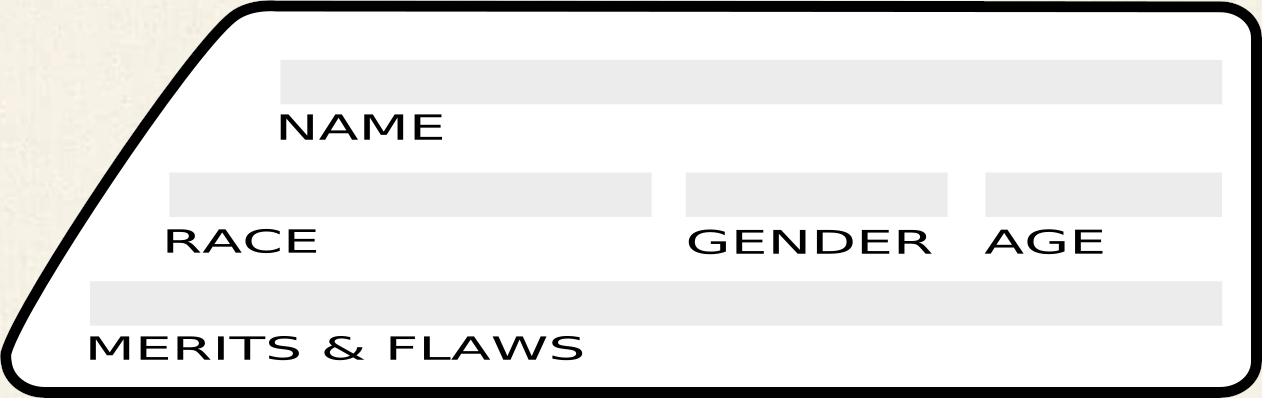
\includegraphics[width=0.95\textwidth]{images/character_base_stats}
    \medskip   
\end{column}

Name, Geschlecht, Rasse, Alter k"onnen durch den Spieler frei gew"ahlt werden. Die Charaktere werden "ublichereise zwischen 30 und 50 Jahre alt sein. Ein deutlich niedriges oder deutlich h"oheres Alter kann negative Einfl"usse auf k"orperliche Fitness oder F"ahigkeiten des Charakters haben. Eine entsprechende Einschr"ankung kann unter Schw"achen auf dem Charakerblatt notiert werden. Um die Charaktere dar"uber hinaus lebhafter zu gestalten, kann jeder der Charaktere eine Schw"ache wie Phobie vor gro\3eren Menschenansammlungen, Angst vor engen R"aumen, Sucht nach Aufputschmittel oder Vorurteile gegen Mutanten oder umgekehrt gegen"uber Norms haben.

\begin{column}[l]{0.58}
    Wird der Charakter im Kampf oder bei einer sonstigen T"atigkeit verletzt wird unter Verletzungen die zugezogenen Verletzungen notiert. 
\end{column}
\begin{column}[r]{0.42}
    \centering
    
\includegraphics[width=0.80\textwidth]{images/character_damage}
\end{column}
\smallskip

Die St"arken eines Charakters werden aufgeteilt nach den Attributen K"orper (\emph{[B]ODY}), Empathie (\emph{[E]MPATHY}) und Bildung (\emph{[S]CIENCE}) gruppiert. Der Attribute repr"asentieren die Grundf"ahigkeiten des Charakters. Unter den Attributen sind die St"arken des Charakters aufgeteilt in drei \emph{F"ahigkeiten} gelistet. Neben der F"ahigkeiten sind jeweils die Anzahl der W"urfel notiert die f"ur eine Aktionen zur Verf"ugung stehen. Die ausgef"ullte Checkbox neben einem Attribut gibt an, dass f"ur eine Grundf"ahigkeit jeweils ein W"urfel zur Verf"ugung steht. F"ur F"ahigkeiten eines Charakters stehen bis zu drei W"urfel zur Verf"ugung die durch die Checkboxen neben den St"arken festgehalten werden. Ein markiertes Dreiecke rechts neben einem Attribut markiert ein Attribut bei dem f"ur F"ahigkeiten bis zu drei W"urfel zur Verf"ugung stehen. Bei Mutanten liegen die F"ahigkeiten f"ur die bis zu drei W"urfel zur Verf"ugung stehen auf dem Attribute K"orper. Norms k"onnen frei zwischen Empathie und Bildung w"ahlen. F"ur F"ahigkeiten k"onnen insgesamt 6 Punkte vergeben werden.
Die F"ahigkeiten eines Charakters beziehen sich immer auf einen entsprechenden Hintergrund. Die Eigentschaft Geschicklichkeit eines Piloten erlaubt bei dem Bedienung eines Raumschiffes oder bei einem Raumspaziergang mehr als einen W"urfel zu werfen w"ahrend ein Schiffstechniker Reparaturen und Modifikationen an einem Schiff mit den W"urfeln durchf"uhren kann. In wie weit eine F"ahigkeit auf eine Aktion angewendet werden kann liegt im Ermessen des Spielleiters. Die F"aihigkeiten sind bewusst grob gew"ahlt und "uberschneiden sich in teilen. Welche F"ahigkeit jeweils angewendet werden kann ergibt sich aus der Aktion die ein Spieler durchf"uhrn will.

\begin{column}[l]{0.55}
    F"ur das Attribut K"orper stehen die Eigenschaften:

    \begin{description}
        \item[Kampf (\emph{Fight})] Kampf wird im Falle von Mann zu Mann Nah-- oder Fernk"ampfen angewendet. Der Hintergrund bestimmt in 
            welcher Kampfart und mit welchen Waffen ein Charakter ausgebildet oder ge"ubt ist.
        \item[Sportlichkeit (\emph{Agility})] Sportlichkeit umfasst Sportlichkeit und Fingerfertigkeiten.
        \item[Geschicklichkeit (\emph{Dexterity})] Geschicklichkeit umfasst handwerkliche F"ahigkeiten im Kontext der Ausbildung eines 
            Charakters.
    \end{description}
\end{column}
\begin{column}[r]{0.45}
    \centering
    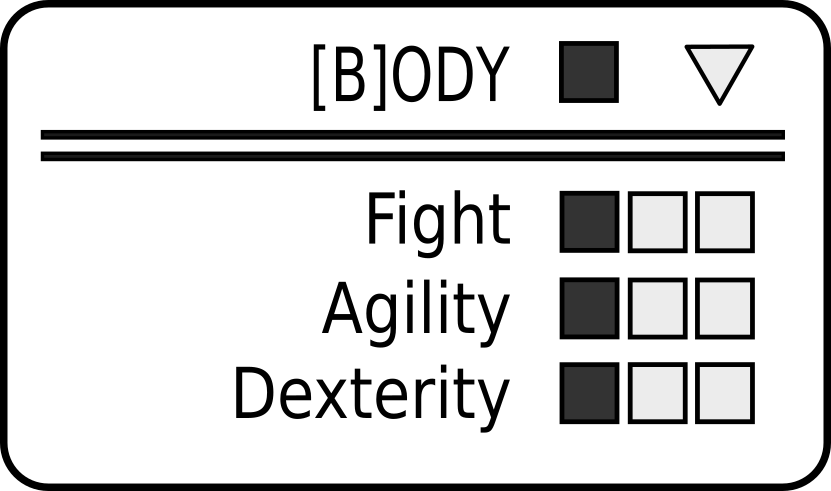
\includegraphics[width=0.80\textwidth]{images/character_body}
\end{column}

Bei schwerwiegenden Verletzungen ist ein Konstitutionswurf notwendig damit der Charakter bei Bewusstseins bleibt. Details finden sich im Kapitel "'Kampf"'.

\begin{column}[l]{0.52}
    F"ur eine Szene stehen dem Charakter 4 Schicksalspunkte (\emph{FATE}) zur Verf"ugung. Ausgegebene Schicksalspunkte werden unter Fate abgestrichen.
\end{column}
\begin{column}[r]{0.48}
    \centering
    
\includegraphics[width=0.80\textwidth]{images/character_fate}    
\end{column}

\begin{column}[l]{0.52}
    Die im Kapitel "`Der Charakter"' Hintergr"unde des Charakters werden im Feld \emph{Back Ground} notiert. Hintergr"unde sind jeweils einem der Attribute Body, Emphathy und Science zugeordnet. Sind unter dem entsprechenden Attribut Punkte f"ur St"arken 
\end{column}
\begin{column}[r]{0.48}
    \centering
    
\includegraphics[width=0.80\textwidth]{images/character_background}    
\end{column}

  

\newsection{Rassenbesonderheiten}

Den Spieler stehen \emph{Norms}, \emph{Alpha Mutanten} und \emph{Omega Soldaten} zu Auswahl. Bez"uglich dem Regelwerte gelten folgende Besonderheiten.

\begin{description}
    \item[Norms] Norms sind normale Menschen, im Falle der Charaktere gebildete Menschen mit einer Hochschulbidung im Zivilen oder 
        milit"arischen Sektor. Ihr m"ogliche St"arke liegt dadurch im Sektor \emph{Science}. In diesem Bereich k"onnen bis zu zwei Punkte bei den F"ahigkeiten vergeben werden. Die Charaktere werden k"onnen in ihrer Laufbahn eine leitende Stelle eingenommen haben und werden von Konzernmitarbeitern als Ansprechpartner wahrgenommen. Die Charaktere h"atten die M"oglichkeit hochwertige K"orpermodifikationen durchf"uhren zu lassen. Norms besitzen einen familier"aren Hintergrund auch wenn der Kontakt abgebochen ist bestehen wenn n"otig Kontakte aus Schulzeit und Hochschulzeiten.
    \item[Alpha Mutanten] Alphas sind in einer Zuchtfarm auf dem Mars als Arbeiter ausgebildet worden. Die geh"oren der
        Arbeiterklasse an. Sie sind handwerklich gut ausgebildet. Aufgrund ihres genetischen Zuchtmaterials sind sie gr"o\3er, st"arker und widerstandsf"ahiger wie Norms. Bei k"orperlichen T"atigkeiten wie auch bei K"orperbelastungen sollten diese k"orperlichen Besonderheiten bei den Auswirkungen von Aktionen ber"ucksichtigt werden. Die m"ogliche St"arke der Alpha Mutanten liegt damit auf den \emph{Body} Werten. Bei den entsprechenden F"ahigkeiten k"onnen dadurch jeweils bis zu zwei Punkte ausgegeben werden. Alpha Mutanten werden als Teil der zivielen Gesellschaft wahrgenommen und werden aufgrund ihrer meist umg"anglichen Art im extraterrestrischen Umfeld freundschaftlich und als zuverl"assig behandelt. Alpha Mutanten sind im Normalfall mit dem Leben in Schwerelosigkeit vertraut und haben oft eine Ausbildung als Piloten f"ur Pods und Drohnen. Alphas haben eine handwerkliche und meist eine logistische Ausbildung erhalten. Alpha Mutanten haben innerhalb ihrer Zuchtreihe jeweils eine eigene Sprache erhalten und k"onnen sich damit mit ihren "`Verwandten"' aber auch anderen Alpha Mutanten unverst"andlich f"ur Norms und Omega Mutanten unterhalten. 
    \item[Omega Mutanten] Omega Mutanten sind entweder auf dem Mars oder in Zuchtfarmen im erdnahen Orbit aufgewachsen. Sie sind deutlich   
        gr"o\3er, st"arker und wiederstandsf"ahiger wie Alpha Mutanten und Norms. Bei allen k"orperlichen Aktionen und Folgen von Verletzungen m"ussen diese "uberlegenen Eigenschaften ber"ucksichtigt werden. Ihre St"arke im W"urfelsystem liegt wie bei Alpha Mutanten im Bereich der \emph{Body} Werte. Hier k"onnen auf alle F"ahigkeiten bis zu zwei Punkte vergeben werden. Omega Soldaten werden von klein auf auf den Krieg vorbereitet und ausgebildet. Nah-- und Fernkampff"ahigkeiten sind vorrauszusetzen. Omega Mutanten sind mit milit"richen K"orpermodifikationen aisgestattet. Omega Mutanten haben eine strategische und logistische Ausbildung f"ur Kriesensituationen erhalten. Sie sind f"ur die m"uhelose Bewegung in Schwerelosigkeit vorbereitet. Sie haben eine medizinische Ausbildung als Sanit"ater. Viele Omega Mutanten sind ausgebildete Piloten oder haben eine Ausbildung als Schiffskomandant absolviert. Aufgrund ihrer genetischen Programmierung sind Omega Mutanten leicht reizbar und gehen schnell offensiv mit einer provokation oder einer Bedrohung um. Sie unterliegen deshalb dem \emph{Flaw} "`reizbar"'. Von nicht Omega Mutanten werden sie oft als militanten Bedrohung wahrgenommen.
\end{description}

\newsection{Kampf}

\begin{remarks}
    Hektor und der Minenarbeiter Fury ein kr"aftiger Alpha Mutant sind sich ins Gehege gekommen. Fury schl"agt zu.

\end{remarks}


\pageimage{images/character_sheet}
